%Dokumentklasse
\documentclass[a4paper,12pt]{scrreprt}
\usepackage[left= 3cm,right = 3cm, bottom = 3 cm]{geometry}
%\usepackage[onehalfspacing]{setspace}
% ============= Packages =============

% Dokumentinformationen
\usepackage[
	pdftitle={Website-Penetration Testing},
	pdfsubject={},
	pdfauthor={Euer Name},
	pdfkeywords={},	
	%Links nicht einrahmen
	hidelinks
]{hyperref}


% Standard Packages
\usepackage[utf8]{inputenc}
\usepackage[ngerman]{babel}
\usepackage[T1]{fontenc}
\usepackage{graphicx, subfig}
\graphicspath{{img/}}
\usepackage{fancyhdr}
\usepackage{lmodern}
\usepackage{color}
\usepackage[export]{adjustbox}
\usepackage{setspace}
\usepackage{float}


% zusätzliche Schriftzeichen der American Mathematical Society
\usepackage{amsfonts}
\usepackage{amsmath}

%nicht einrücken nach Absatz
%\setlength{\parindent}{0pt}


% ============= Kopf- und Fußzeile =============
\pagestyle{fancy}
%
\lhead{}
\chead{}
\rhead{\slshape \leftmark}
%%
\lfoot{}
\cfoot{\thepage}
\rfoot{}
%%
\renewcommand{\headrulewidth}{0.4pt}
\renewcommand{\footrulewidth}{0pt}

% ============= Package Einstellungen & Sonstiges ============= 
%Besondere Trennungen
\hyphenation{De-zi-mal-tren-nung}


% ============= Dokumentbeginn =============

\begin{document}
%Seiten ohne Kopf- und Fußzeile sowie Seitenzahl
\pagestyle{empty}

\begin{center}
\begin{tabular}{p{\textwidth}}



\includegraphics[scale=0.5, right]{img/dhbw-logo.png}


\\

\begin{center}
\LARGE{\textsc{
Ethical Hacking:\\
Website-Penetration Testing \\
}}
\end{center}

\\


\begin{center}\large
    { im Studiengang}
\end{center}

\\

\begin{center}\large
    { Informatik Cybersecurity}
\end{center}

\begin{center}
an der dualen Hochschule Baden-Württemberg Mannheim
\end{center}


\begin{center}
von
\end{center}


\begin{center}
    \begin{tabular}{lll}
    \textbf{Name, Vorname:} & & Hartinger, Steven\\
    \textbf{Abgabedatum:} & & 01.09.2022\\
    \end{tabular}
    \end{center}

\\

\\

\begin{center}
\begin{tabular}{lll}
\textbf{Bearbeitungszeitraum:} & & 27.06.2022 - 01.09.2022\\
\textbf{Matrikelnummer, Kurs:} & & 7146735, TINF20CS1\\
\textbf{Ausbildungsunternehmen} & & MLP Finanzberatung SE\\
\textbf{Betrieblicher Betreuer:} & & Sebastian Damm\\

\\
\\


\end{tabular}
\end{center}

\end{tabular}
\end{center}

%Inhaltsverzeichnis
\tableofcontents

\chapter{Executive Summary}
\section*{Synopsis}
\hfill\break

As part of the lecture ''Offensive Security'' by Dr. Prof. Bauer the students of the TINF20CS1 performed a review on a Raspberry Pi handed by our lecturer. The objective of this task is to prepare a report on penetration testing for a Raspberry Pi B3+. The Raspberry Pi B3+ is powered by a 64-bit quad-core ARM Cortex-A53 CPU operating at 1.4GHz and has 1GB of LPDDR2 RAM. Its 40-pin GPIO header allows users to connect a diverse range of sensors and actuators, making it an excellent tool for development and learning. The device provided for this assignment comes with a 16GB microSD card, a 5V 2.5A power supply connected to a Micro-USB Cable, and a case. Our aim is to assess the security of the \ac{DUT}, including its OS and services, without prior knowledge of the specifics.
\section*{Scope}
\hfill \break

Our assessment included:
\begin{itemize}
    \item Validation of the given Raspberry Pi without exact requirements. 
    \item Provide countermeasures for vulnerablities of the system.
\end{itemize}

The threats included:
\begin{itemize}
    \item Network Eavesdrop - The attacker is on a wireless communication channel or somewhere else on the network
    \item Network Attack - The attacker is on a wireless communication channel or somewhere else on the network
    \item Physical Access - The attacker has physical access to the device
    \item Malicious Code - Malicious code loaded onto the Raspberry Pi
\end{itemize}

Testing was performed on:
\begin{itemize}
    \item Raspberry Pi 3
\end{itemize}

\section*{Limitations}
\section*{}

For this assessment we are not having any limitation besides a time limit.
\section*{Key Findings}
\hfill\break

This penetration test report revealed a significant number of critical findings that require immediate action to prevent potential security breaches. The test identified a total of 22 findings, including unauthorized access to the Device Under Test (DUT) and several misconfigurations that could be exploited by attackers. \\
Based on these findings, urgent action is required to address the vulnerabilities and mitigate potential risks. We recommend implementing a comprehensive security program that includes regular patching, strong authentication controls, and network segmentation to limit access to sensitive resources.\\
Furthermore, it is crucial to review and update security policies and procedures to ensure they align with industry standards and best practices. Regular security training for staff and users is also necessary to raise awareness and promote good security practices.\\
In conclusion, this report highlights security risks and vulnerabilities present in the DUT. It is essential to take immediate action to address these issues and implement a comprehensive security program to ensure the confidentiality, integrity, and availability of sensitive data and systems.


\chapter*{Dashboard}
\label{sec:dashboard}

\section*{Target Metadata}

\section*{Targets}

\section*{Finding Breakdown}

\section*{Category Breakdown}




\chapter*{Findings}
\begin{table}[htb]
    \renewcommand{\arraystretch}{1.5}
    \begin{tabular*}{\textwidth}{|>{\columncolor{orange!15}}p{3cm}|p{17.1cm}|}
    \textbf{Finding} & \textbf{Path Traversal}\\
    Risk& Medium\\
    Category&Access Controls\\
    Impact& An attacker could access sensitive data. This can also happen with any user by accident. \\ \\
    Description& After performing an nmap scan three open ports where found. Since there is most likely a \ac{http} service running on port 80 a http-enum script was used to try to access several potentially interesting paths.
    \newline
    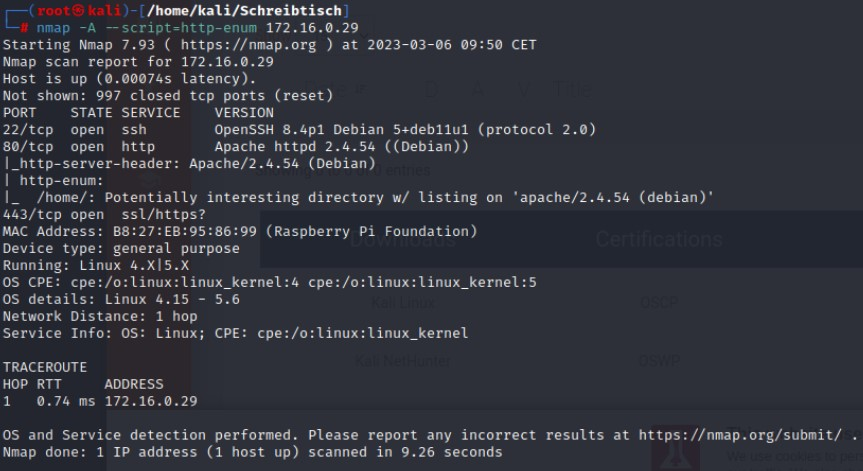
\includegraphics[width = 0.73\textwidth]{http_vulnerbility.jpg}
    \newline
    The script was able to access the ''/home'' path where the apache server has its directories saved. In this case no sensitive files were found. 
    \\&
    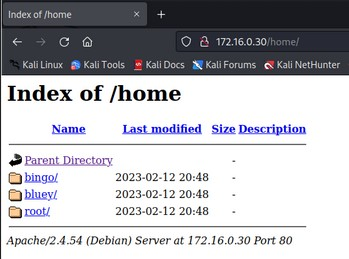
\includegraphics[width = 0.5\textwidth]{dateisystem.jpg} \\
    Recommendation&\\
    \end{tabular*}
    \end{table}
% Beendet eine Seite und erzwingt auf den nachfolgenden Seiten die Ausgabe aller Gleitobjekte (z.B. Abbildungen), die bislang definiert, aber noch nicht ausgegeben wurden. Dieser Befehl fügt, falls nötig, eine leere Seite ein, sodaß die nächste Seite nach den Gleitobjekten eine ungerade Seitennummer hat. 
\cleardoubleoddpage

% pagestyle für gesamtes Dokument aktivieren
\pagestyle{fancy}

%Literaturverzeichnis
\bibliographystyle{unsrtdin}
\bibliography{Literatur}

\end{document}
